%%%%%%%%%%%%%%%%%%%%%%%%%%%%%%%%%%%%%%%%%%%%%%%%%%%%%%%%%%%%%%%%%%%%%%
% Lớp 11 | Đường thẳng, mặt phẳng. Quan hệ song song trong | Phép chiếu song song
% Dạng 1H4?6-5: Tính tỉ số đoạn thẳng, diện tích qua phép chiếu
% Số câu: 22  (sinh tự động bởi tach_cau.py; từ nay thầy sửa trực tiếp file này)
%%%%%%%%%%%%%%%%%%%%%%%%%%%%%%%%%%%%%%%%%%%%%%%%%%%%%%%%%%%%%%%%%%%%%%

%%%%%%%%%%%%%%%% TRẮC NGHIỆM 4 PHƯƠNG ÁN %%%%%%%%%%%%%%%%

% nguồn: Ok_Toan11_TracNghiem_Lan2
\begin{ex}%[1H4V6-5]%[ma:8f7f6e67]
	\immini{Cho hình chóp $S.ABCD$ có đáy $ABCD$ là hình bình hành. Gọi $M$ là điểm thuộc cạnh $SD$ sao cho $SM=\dfrac{2}{3}SD$. Mặt phẳng chứa $AM$ và song song với $BD$ cắt cạnh $SC$ tại  $K$. Tỷ số $\dfrac{SK}{SC}$ bằng
	 \choice
		 {$\dfrac{1}{3}$}
		{$\dfrac{2}{3}$} 
		{\True  $\dfrac{1}{2}$}
		{$\dfrac{3}{4}$}}{\begin{tikzpicture}
		\tikzset{declare  function={a=4; b=2; h=3.5;}}
		\path (0,0) coordinate (A) 
			(a,0)  coordinate (D)
			(-135:b) coordinate  (B)
			 ($(B)+(D)$) coordinate (C)
			(0,h) coordinate  (S)
			 ($(S)!2/3!(D)$) coordinate (M);
		\path  pic[draw,angle radius=5pt]{right angle=B--A--S};
		\path pic[draw,angle  radius=5pt]{right angle=D--A--S};
		 \draw[dashed] (B)--(A)--(D)
			(A)--(S) 
			(A)--(M); 
		\draw  (S)--(B)--(C)--(D)--cycle (S)--(C);
		\foreach \t/\g in  {A/180,B/-90,C/-90,D/90,S/90,M/90}{
			\draw[fill=black]  (\t) circle (1pt) node[shift={(\g:9pt)},font=\scriptsize]{$\t$};
		 }
	\end{tikzpicture}
		 }
	 \loigiai{
	\immini{Nối  $BD$.\\
		Trong mặt phẳng $(SBD)$  qua $M$ vẽ đường thẳng song song với $BD$ cắt $SB$ tại $N$.\\
		Trong mặt phẳng  $(ABCD)$, gọi $O=AC\cap BD$.\\
		Trong mặt  phẳng $(SBD)$, gọi $I=SO\cap MN$.\\
		 Trong mặt phẳng $(SAC)$, gọi $K=AI\cap SC\\\Rightarrow\heva{&K\in AI\subset(AMN)\\&K\in SC}\Rightarrow K=SC\cap(AMN)$.\\
		$\triangle SOD$  có $MI\parallel DO\Rightarrow\dfrac{SI}{SO}=\dfrac{SM}{SD}=\dfrac{2}{3}$.\\
		Xét $\triangle SAC$ có $SO$ là  trung tuyến và $\dfrac{SI}{SO}=\dfrac{2}{3}\\\Rightarrow I$ là trọng tâm tam giác $\triangle SAC$.\\
		 Suy ra $AK$ là đường trung tuyến của $\triangle SAC$.\\
		Do đó $K$ là trung điểm của $SC\Rightarrow\dfrac{SK}{SC}=\dfrac{1}{2}$.}{\begin{tikzpicture}
		\tikzset{declare  function={a=4; b=2; h=3.5;}}
		\path  (0,0) coordinate (A)
			(a,0) coordinate  (D)
			(-135:b) coordinate (B) 
			($(B)+(D)$) coordinate (C) 
			 (0,h) coordinate (S)
			 ($(S)!2/3!(D)$) coordinate (M)
			($(S)!2/3!(B)$)  coordinate (N)
			(intersection  of A--C and B--D) coordinate (O)
			(intersection of  M--N and S--O) coordinate (I)
			(intersection of A--I and S--C) coordinate (K); 
		\draw[dashed]  (B)--(A)--(D)
			(A)--(S) 
			 (A)--(C)
			(B)--(D) 
			 (A)--(M)
			(S)--(O) 
			 (M)--(N)
			(A)--(K); 
		 \draw (S)--(B)--(C)--(D)--cycle (S)--(C);
		\foreach  \t/\g in {A/180,B/-90,C/-90,D/90,S/90,O/-90,M/90,I/150,K/40}{
			\draw[fill=black] (\t) circle (1pt)  node[shift={(\g:9pt)},font=\scriptsize]{$\t$};
		} 
	\end{tikzpicture}
		} 
	} 
\end{ex}

% nguồn: Ok_Toan11_TracNghiem_Lan2
\begin{ex}%[1H4V6-5]%[ma:2d2bb4c7]
	Cho hình chóp $S.ABCD$ có đáy là hình bình hành. Gọi $M$ là trung điểm của $SD$, $G$ là trọng tâm tam giác $SAB$, $K$ là giao điểm  của $GM$ với mặt phẳng $ABCD$. Tỉ số $\dfrac{KB}{KC}$ bằng
	\choice 
		 {$\dfrac{2}{3}$}
		 {$2$}
		{\True $\dfrac{1}{2}$} 
		 {$\dfrac{3}{2}$}
	\loigiai{ 
		\begin{center}
			\begin{tikzpicture}[declare function={gocx=90; goc=-150; a=5; b=a/2; h=4;}]
					\path (0,0)  coordinate (A)--+(gocx:h) coordinate (S)
						 (a,0) coordinate (D)
						(goc:b)  coordinate (B)
						 +(a,0) coordinate (C)
						($(A)!0.5!(B)$)  coordinate (N)
						($(S)!0.5!(D)$) coordinate (M) 
						($(S)!2/3!(N)$)  coordinate (G)
						(intersection of B--C and N--D)  coordinate (K)
						(intersection of M--G and S--B) coordinate  (J)
						(intersection of D--N and  S--B) coordinate (L);
					 \draw[dashed] (S)--(A)
						(B)--(A)--(D) 
						 (S)--(N)
						 (A)--(M)
						(M)--(J) 
						(N)--(L) 
						 (N)--(D);
					\draw (S)--(B)--(C)--(S)--(D)--(C)--cycle (J)--(K) 
						 (B)--(K)
						(L)--(K); 
					\foreach  \x/\goc in {S/90,A/150,D/0,C/-60,B/-90,N/-90,M/90,G/-60,K/180}
					 \draw[fill=black] (\x) node[shift={(\goc:7pt)},font=\scriptsize]{$\x$} circle (1pt);
				\end{tikzpicture}
		\end{center}
		Gọi $N$ là  trung điểm của $AB$.\\
		Trong  mặt phẳng $(SDN)$, $GM\cap DN=K$.\\
		Ta có $\heva{&K\in GM\\&K\in  DN\subset(ABCD)}\Rightarrow GM\cap(ABCD)=K$.\\
		Áp dụng định lý Menelaus cho tam giác $SND$  với ba điểm $M$, $G$, $K$ thẳng hàng ta có \[\dfrac{NK}{KD}\cdot\dfrac{DM}{MS}\cdot\dfrac{SG}{GN}=1\Leftrightarrow\dfrac{NK}{KD}\cdot 1\cdot 2=1\Leftrightarrow\dfrac{NK}{KD}=\dfrac{1}{2}.\]
		Suy ra $N$ là trung điểm của  $KD$.\\
		Mà $N$ cũng là trung điểm của $AB$ nên tứ giác $ADBK$ là hình bình hành.\\ 
		Vậy  $KB=AD=BC\Rightarrow\dfrac{KB}{KC}=\dfrac{1}{2}$.
	} 
\end{ex}

% nguồn: Ok_Toan11_TracNghiem_Lan2
\begin{ex}%[1H4V6-5]%[ma:ca283972]
	Cho hình chóp $S.ABCD$ có đáy $ABCD$ là hình bình hành tâm $O$. Gọi $M$ là trung  điểm $AO$. Mặt phẳng $(\alpha)$ qua $M$ và song song với $BD$; $SA$ và mặt phẳng $(\alpha)$ cắt $SC$ tại $N$. Khẳng định nào sau đây là khẳng định đúng?
	 \choice
		 {$SN=\dfrac{1}{4}NC$}
		 {$SN=NC$}
		 {\True $SN=\dfrac{1}{3}NC$}
		{$SN=\dfrac{1}{2}NC$} 
	 \loigiai{
	 \immini{Vì
		 $\heva{&SA\parallel(\alpha)\\&(SAC)\cap(\alpha)=MN}\Rightarrow MN\parallel SA$.\\
		Xét $\triangle SAC$ với $MN\parallel SA$ nên theo định lý  Thalès ta có \[\dfrac{SN}{NC}=\dfrac{AM}{MC}.\]
		Mặt khác do tứ giác $ABCD$ là  hình bình hành tâm $O$ kết hợp với $M$ là trung điểm $AO$ nên suy ra được
		$\dfrac{SN}{NC}=\dfrac{AM}{MC}=\dfrac{1}{3}$.}{ 
		\begin{tikzpicture}[declare function={gocx=80; goc=-140; a=4; b=a/2; h=3;}]
				\path (0,0) coordinate  (A)--+(gocx:h) coordinate (S)
					(a,0) coordinate (D) 
					(goc:b)  coordinate (B)
					+(a,0) coordinate  (C)
					(intersection of A--C and B--D) coordinate  (O)
					($(A)!0.5!(O)$)  coordinate (M)
					 ($(S)!0.25!(C)$) coordinate (N)
					($(A)!0.5!(B)$)  coordinate (E)
					($(A)!0.5!(D)$) coordinate  (F)
					($(S)!0.5!(B)$) coordinate  (P)
					($(S)!0.5!(D)$)  coordinate (Q);
				\draw[dashed] (S)--(A) 
					 (B)--(A)--(D)
					(A)--(C) 
					 (B)--(D)
					 (M)--(N);
				\draw (S)--(B)--(C)--(S)--(D)--(C)--cycle; 
				\fill[gray!30,opacity=0.5] (E)--(P)--(N)--(Q)--(F)--cycle; 
				\draw (P)--(N)--(Q); 
				 \draw[dashed] (Q)--(F)--(E)--(P)
					 (E)--(F);
				\foreach \x/\goc  in {S/90,A/150,B/180,C/-60,D/0,O/-90,M/-90,N/50}
				 \draw[fill=black] (\x) node[shift={(\goc:7pt)},font=\scriptsize]{$\x$} circle (1pt);
			\end{tikzpicture}
		} 
	 }
\end{ex}

% nguồn: Ok_Toan11_TracNghiem_Lan2
\begin{ex}%[1H4V6-5]%[ma:fa9ddad2]
	 Cho hình chóp $S.ABCD$ có đáy $ABCD$ là hình bình hành. Gọi $M$ là trung điểm $SC$, $F$ là giao điểm của đường thẳng $SD$ với mặt phẳng $(ABM)$. Tính tỉ số $\dfrac{SF}{SD}$.
	\choice 
		{$1$} 
		{$\dfrac{1}{3}$} 
		 {$\dfrac{2}{3}$}
		 {\True $\dfrac{1}{2}$}
	\loigiai{ 
	\immini{Chọn  mặt phẳng $(SBD)$ chứa $SD$.\\
		 Tìm giao tuyến của mặt phẳng $(SBD)$ và mặt phẳng $(ABM)$.\\
		Lấy điểm $B\in(SBD)\cap(ABM)$  và gọi $O=AC\cap BD$.\\
		Trong mặt phẳng $(SAC)$, gọi $E=AM\cap SO$ thì ta có \begin{eqnarray*}
		 &&\heva{&E\in AM, AM\subset(ABM)\\&E\in SO, SO\subset(SBD)}\\
		 &\Rightarrow& E\in(SBD)\cap(ABM)\\
		&\Rightarrow&  BE=(SBD)\cap(ABM).
	\end{eqnarray*}}{\begin{tikzpicture}
		\tikzset{declare function={a=4; b=2;  h=3.5;}}
		\path (0,0) coordinate  (A)
			(a,0) coordinate (D) 
			 (-120:b) coordinate (B)
			($(B)+(D)$) coordinate (C) 
			(0,h) coordinate  (S)
			($(S)!0.5!(D)$) coordinate  (F)
			 ($(S)!0.5!(C)$) coordinate (M)
			(intersection  of A--C and B--D) coordinate (O)
			(intersection of A--M and  S--O) coordinate (E);
		 \draw[dashed] (B)--(A)--(D)
			(A)--(S) 
			(A)--(C) 
			(B)--(D) 
			 (S)--(O)
			 (A)--(M)
			(B)--(F) 
			 (B)--(M);
		\draw (S)--(B)--(C)--(D)--cycle  (S)--(C);
		\foreach \t/\g in {A/180,B/-90,C/-90,D/90,S/90,M/0,F/90,O/-90,E/180}{ 
			\draw[fill=black] (\t) circle  (1pt) node[shift={(\g:9pt)},font=\scriptsize]{$\t$};
		 }
	\end{tikzpicture}
	 }
	\noindent Trong mặt phẳng $(SBD)$, gọi $F=SD\cap BE$ thì $\heva{&F\in SD\\&F\in BE, BE\subset(ABM)}\Rightarrow  F=SD\cap(ABM)$.\\
	Vì $O$ là trung điểm $AC$, $M$ là trung điểm $SC$ nên $E$ là  trọng tâm của $\triangle SAC$.\\
	 Suy ra $\dfrac{SE}{SO}=\dfrac{2}{3}$.\\
	Trong $\triangle SBD$ có $SO$ là trung tuyến và $\dfrac{SE}{SO}=\dfrac{2}{3}$ nên $E$ là trọng tâm  của $\triangle SBD$.\\
	Suy ra $BF$ là trung tuyến của $\triangle SBD$.\\ Do đó $F$ là trung điểm  $SD$.\\
	Vậy  $\dfrac{SF}{SD}=\dfrac{1}{2}$.
 }
\end{ex}

% nguồn: Ok_Toan11_TracNghiem_Lan2
\begin{ex}%[1H4V6-5]%[ma:511a2533]
	Cho  hình chóp $S.ABCD$ có đáy là hình bình hành tâm $O$, $M$ là một điểm thuộc đoạn $SA$ sao cho $2MA=SM$, điểm $N$ là điểm thuộc tia đối của tia $OS$ sao cho $3ON=SO$, $G$ là trọng tâm của $\triangle SCD$. Gọi $K=SD\cap(GMN)$. Biết rằng $\dfrac{SK}{KD}=\dfrac{a}{b}$ ($a$, $b\in\mathbb{N}$) và $(a,b)=1$. Tính $S=a+b$.
	\choice 
		{\True  $3$}
		{$2$} 
		{$4$} 
		{$5$} 
	 \loigiai{
		\begin{center}
			\begin{tikzpicture}[declare function={gocx=80; goc=-140; a=4; b=a/2; h=3;}]
					\path (0,0)  coordinate (A)--+(gocx:h) coordinate (S)
						(a,0)  coordinate (D)
						(goc:b) coordinate (B) 
						+(a,0) coordinate (C) 
						(intersection of A--C and  B--D) coordinate (O)
						($(S)!2/3!(A)$) coordinate  (M)
						($(S)!4/3!(O)$)  coordinate (N)
						 ($(C)!0.5!(D)$) coordinate (J)
						($(S)!2/3!(J)$) coordinate  (G)
						($(M)!3/4!(N)$)  coordinate (E)
						(intersection of M--N and A--C) coordinate (F) 
						($(S)!1/3!(D)$)  coordinate (K)
						($(S)!0.5!(C)$)  coordinate (I);
					\draw[dashed] (S)--(A) 
						 (B)--(A)--(D)
						 (A)--(C)
						 (B)--(D)
						 (S)--(N);
					 \draw (S)--(B)--(C)--(S)--(D)--(C)--cycle;
					\draw  (S)--(J);
					 \draw[blue] (E)--(N);
					\draw[dashed,blue]  (G)--(M)
						 (O)--(E)
						(M)--(E) 
						(G)--(N); 
					\draw (G)--(I); 
					\draw[red]  ($(K)!-0.8!(G)$) node[above,font=\scriptsize,black]{$x$}
						 -- ($(G)!-0.8!(K)$) node[below,font=\scriptsize,black]{$x'$};
					\foreach  \x/\goc in {
						S/90, 
						 A/130,
						 B/180,
						C/0, 
						 D/0,
						 O/45,
						M/170, 
						N/-90, 
						 G/-20,
						 E/190,
						F/-150, 
						 K/45,
						I/30, 
						J/0 
					 }
					\draw[fill=black]  (\x) circle (1.2pt) node[shift={(\goc:9pt)},font=\scriptsize]{$\x$};
				\end{tikzpicture}
		\end{center}
		Trong $(SAC)$ từ $O$ dựng đường thẳng $d$ song song với $SA$ cắt $MN$  tại $E$.\\
		Ta có $OE\parallel SM\Rightarrow\dfrac{OE}{SM}=\dfrac{ON}{SN}=\dfrac{1}{4}\Rightarrow\dfrac{OE}{2MA}=\dfrac{1}{4}\Rightarrow\dfrac{OE}{MA}=\dfrac{1}{2}$.\\ 
		Trong $(SAC)$ gọi  $F=MN\cap AC$ ta có $OE\parallel MA\Rightarrow\dfrac{OE}{MA}=\dfrac{OF}{AF}=\dfrac{1}{2}\Rightarrow\dfrac{AF}{AO}=\dfrac{2}{3}\Rightarrow\dfrac{AF}{AC}=\dfrac{1}{3}$.\\
		Ta có $\dfrac{AM}{SA}=\dfrac{AF}{AC}=\dfrac{1}{3}\Rightarrow MN\parallel  SC$.\\
		Ta có $\heva{&G\in(GMN)\cap(SCD)\\&MN\parallel SC\\&MN\subset(GMN), SC\subset(SCD)}\Rightarrow\heva{&xGx'=(GMN)\cap(SCD)\\&xGx'\parallel SC\parallel  MN.}$\\
		 Gọi $K=xGx'\cap SD\Rightarrow\heva{&K\in xGx', xGx'\subset(GMN)\\&K\in SD}\Rightarrow K=SD\cap(GMN)$.\\
		Ta có  $GK\parallel SC\Rightarrow\dfrac{DK}{SD}=\dfrac{DG}{DI}=\dfrac{2}{3}\Rightarrow\dfrac{SK}{KD}=\dfrac{1}{2}\Rightarrow \heva{&a=1\\&b=2}\Rightarrow a+b=3$.
	} 
\end{ex}

% nguồn: Ok_Toan11_TracNghiem_Lan2
\begin{ex}%[1H4V6-5]%[ma:64ed1285]
	Cho hình chóp $S.ABC$ có $G$, $K$ lần lượt là trọng tâm của các tam giác $ABC$ và $SBC$, gọi $E$ là trung điểm của $AC$. Mặt phẳng $(GEK)$ cắt $SC$ tại $M$.  Tỉ số $\dfrac{MS}{MC}$ bằng
	\choice 
		 {\True $1$}
		 {$2$}
		{$\dfrac{2}{3}$} 
		 {$\dfrac{1}{2}$}
	\loigiai{ 
	\immini{Gọi $N$ là  trung điểm của $BC$.\\
		Theo đầu bài ta có $G$, $K$ lần lượt là trọng tâm của  các tam giác $ABC$ và $SBC$ nên ta có \[\dfrac{NK}{NS}=\dfrac{NG}{NA}=\dfrac{1}{3}\Rightarrow GK\parallel SA\Rightarrow(GEK)\parallel SA.\]
		Từ trên mặt phẳng $(SAC)$, ta dựng đường thẳng đi  qua $E$ và song song với $SA$ cắt $SC$ tại $M$.\\
		Ta  có $\heva{&EM\parallel SA\\&GK\parallel SA}\Rightarrow EM\parallel GK\Rightarrow M\in(EGK)$.\\
		 Vậy $(EGK)\cap SC=M$.\\
		Vì $E$ là trung điểm của $AC$, $EM\parallel SC$  nên $EM$ là đường trung bình của $\triangle SAC$.\\
		Vậy tỉ số $\dfrac{MS}{MC}=1$.}{\begin{tikzpicture}[declare function={goc=-55; a=5; b=0.45*a; h=7;}]
		 \path
			(0,0.5)  coordinate (A)
			(a,0) coordinate  (C)
			(goc:b) coordinate (B)--+(0,h) coordinate  (S)
			 ($(B)!0.5!(C)$) coordinate (N)
			 ($(A)!2/3!(N)$) coordinate (G)
			 ($(A)!0.5!(C)$) coordinate (E)
			($(S)!2/3!(N)$) coordinate  (K)
			($(B)!0.5!(S)$) coordinate  (J)
			($(C)!0.5!(S)$) coordinate (M); 
		\draw[dashed]  (A)--(C)
			(A)--(N) 
			(E)--(G)--(K) 
			 (E)--(M);
		 \draw (S)--(B)
			 (S)--(A)--(B)--(C)--cycle (S)--(N)
			(C)--(J) 
			 (K)--(M);
		 \foreach \x/\goc in {S/90,A/240,C/-60,B/-90,N/-90,G/-90,E/-60,K/200,M/0}
		\draw[fill=black] (\x) node[shift={(\goc:7pt)},font=\scriptsize]{$\x$}  circle (1pt);
	\end{tikzpicture}
		} 
	} 
\end{ex}

% nguồn: Ok_Toan11_TracNghiem_Lan2
\begin{ex}%[1H4V6-5]%[ma:17d724db]
	Cho hình hộp  $ABCD.A'B'C'D'$. Xác định các điểm $M$, $N$ tương ứng trên các đoạn $AC'$, $B'D'$ sao cho $MN$ song song với $BA'$ và tính tỉ số $\dfrac{MA}{MC'}$.
	\choice 
		{\True  $2$}
		{$3$} 
		{$4$} 
		{$1$} 
	\loigiai{ 
	 \immini{
		Xét phép chiếu song song lên mặt phẳng $(A'B'C'D')$ theo  phương chiếu $BA'$.\\
		Ta có $N$ là ảnh của $M$ hay $N$ chính là  giao điểm của $B'D'$ và ảnh $AC'$ qua phép chiếu này.\\
		Do đó ta xác định $M$, $N$  như sau
		\begin{itemize}
			\item Trên $A'B'$ kéo dài lấy điểm $K$ sao cho $A'K=B'A'$ thì  $ABA'K$ là hình bình hành nên $AK\parallel BA'$.
			\item Suy ra  $K$ là ảnh của $A$ trên $A'B'$ qua phép chiếu song song.
			\item Gọi $N=B'D'\cap  KC'$.\\
			Đường thẳng qua $N$ và song song với $AK$ cắt $AC'$ tại $M$. 
		\end{itemize}
		 }{
		\begin{tikzpicture}[scale=0.7,font=\footnotesize,line join=round,line cap=round,>=stealth]
				 \def\bc{4}
				 \def\ba{2.5}
				\def\h{3.7} 
				\def\gocB{100} 
				\coordinate[label=below:$B$] (B)  at (0,0);
				\coordinate[label=above:$A$] (A) at  (\gocB:\ba);
				\coordinate[label=right:$C$]  (C) at (\bc,0);
				 \coordinate[label=above:$D$] (D) at ($(A)+(C)-(B)$);
				\coordinate[label=left:$A'$] (A')  at ($(A)+(-120:\h)$);
				 \coordinate[label=below:$B'$] (B') at ($(B)+(A')-(A)$);
				 \coordinate[label=below:$C'$] (C') at ($(C)+(A')-(A)$);
				\coordinate[label=right:$D'$] (D') at ($(D)+(A')-(A)$); 
				\coordinate[label=right:$M$] (M) at ($(A)!2/3!(C')$); 
				\coordinate[label=above:$K$] (K) at  ($(B')!2!(A')$);
				\coordinate[label=below:$N$] (N)  at ($(K)!2/3!(C')$);
				\draw (A)--(A')--(B')--(C')--(C)--(D)--cycle (B)--(B') 
					(A)--(B)--(C) 
					(A)--(K)--(A')--(B); 
				 \draw[dashed] (A')--(D')--(B')
					 (D)--(D')--(C')--(A)
					(K)--(C') 
					 (M)--(N);
				\foreach \diem in {A,B,C,D,A',B',C',D',M,K,N}  \fill (\diem) circle (1pt);
			\end{tikzpicture}
		 }
		 \noindent
		Ta có $M$, $N$  là các điểm cần xác định.\\
		Theo định lí  Thales, ta có $\dfrac{MA}{MC'}=\dfrac{NK}{NC'}=\dfrac{KB'}{C'D'}=2$.
	} 
\end{ex}


%%%%%%%%%%%%%%%% ĐÚNG/SAI %%%%%%%%%%%%%%%%

% nguồn: Ok_dungsai_lop11_Lan1
\begin{ex}%[1H4H6-5]%[ma:f6e47c96]
 Cho hình chóp $S.ABCD$ có đáy  là hình bình hành, trên cạnh $SA$ lấy điểm $M$ sao cho $MA=2MS$. Gọi $O$ là tâm của hình bình hành $ABCD$. Một phép chiếu song song theo phương $MO$ lên mặt phẳng $(ABCD)$ biến điểm $S$ thành điểm $N$.
 \choiceTF 
  {\True $N$ là hình chiếu song song của $S$ lên mặt phẳng $(ABCD)$ theo phương  $OM$}
   {$\dfrac{AO}{AN}=\dfrac{1}{3}$}
   {$\dfrac{AN}{AC}=4$}
  {\True $\dfrac{CN}{CA}=\dfrac{1}{4}$} 
 \loigiai{\begin{center}
  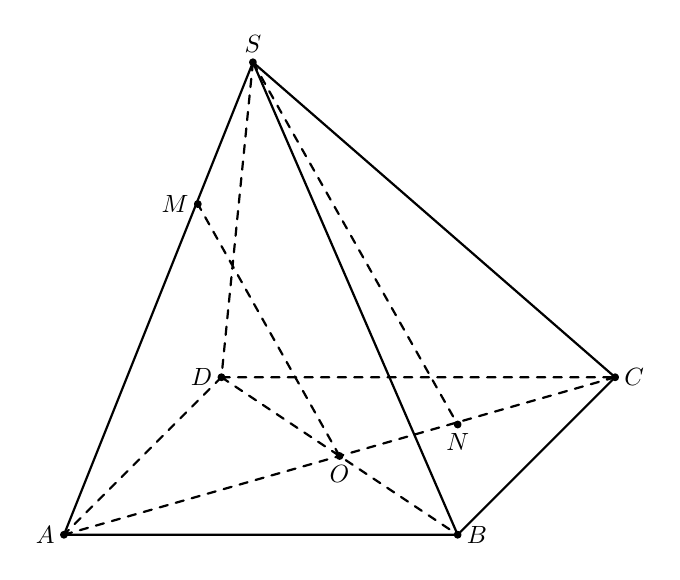
\begin{tikzpicture}[line join=round,line cap=round,>=stealth,thick]
    \coordinate  (A) at (-4,-2);
    \coordinate  (B) at (1,-2);
    \coordinate  (C) at (3,0);
    \coordinate (D) at  (-2,0);
    \coordinate (S) at  (-1.6,4);
     \coordinate (N) at (1,-0.6);
    \coordinate (M) at  (-2.3,2.2);
    \coordinate (O) at (intersection of D--B and  A--C);
     \draw[dashed](S)--(D)
     (D)--(A) 
      (D)--(C)
      (D)--(B)
      (A)--(C)
     (S)--(N) 
      (O)--(M);
     \draw (S)--(A)
     (A)--(B) 
      (S)--(B)
      (S)--(C)
      (B)--(C);
    \foreach \i in {S,A,B,C,D,M,N,O}{\draw[fill=](\i) circle (1pt);} 
    \foreach \i in {S}{\draw (\i) node[scale=0.9,above]{$\i$};} 
     \foreach \i in {M,D,A}{\draw (\i) node[scale=0.9,left]{$\i$};}
    \foreach \i in  {O,N}{\draw (\i) node[scale=0.9,below]{$\i$};}
    \foreach \i in {B,C}{\draw  (\i) node[scale=0.9,right]{$\i$};}
   \end{tikzpicture}
 \end{center}
 \begin{itemchoice}
  \itemch \textbf{Đúng}. Trong mặt phẳng $(SAC)$ kẻ $SN$  song song $OM$ với $N$ thuộc $AC$. Khi đó $N$ thuộc mặt phẳng $(ABCD)$ nên $N$ là hình chiếu song song của $S$ lên mặt phẳng $(ABCD)$ theo phương $OM$.
  \itemch \textbf{sai}. Tam giác $SAN$ có $OM  \parallel SN \Rightarrow \dfrac{AM}{AS}=\dfrac{AO}{AN}=\dfrac{2}{3}.\quad(1)$.
  \itemch \textbf{sai}. Suy  ra $\dfrac{\dfrac{1}{2}AC}{AN}=\dfrac{2}{3} \Rightarrow \dfrac{AC}{AN}=\dfrac{4}{3} \Rightarrow \dfrac{AN}{AC}=\dfrac{3}{4}.\quad(2)$.
  \itemch \textbf{Đúng}. Từ $(1)$, $(2)$ suy ra  $\dfrac{CN}{CA}=\dfrac{1}{4}$.
 \end{itemchoice}
} 
\end{ex}

% nguồn: Ok_dungsai_lop11_Lan1
\begin{ex}%[1H4V6-5]%[ma:23410e78]
 Cho hình chóp $S.ABCD$ có đáy $ABCD$ là hình bình hành tâm $O$. Gọi hai điểm $E, F$ lần lượt trên các cạnh $SB, SC$ sao  cho $\dfrac{SF}{SC}=\dfrac{1}{2}$ và $\dfrac{SE}{SB}=\dfrac{2}{3}$.
  \choiceTF
  {\True Hai mặt phẳng $(AEF)$ và $(ABCD)$ cắt  nhau theo giao tuyến $d$}
  {$BD$ không song  song mặt phẳng $(AEF)$}
  {\True Gọi $J$ là giao điểm  của $SD$ và $(AEF)$. Tỷ số $\dfrac{SJ}{SD}=\dfrac{2}{3}$}
  {\True Ba  đường thẳng $d, JF$ và $CD$ đồng quy}
  \loigiai{
  \begin{center}
   \begin{tikzpicture}[scale=1,font=\footnotesize,line join=round,line cap=round,>=stealth]
      \def\bc{4}
     \def\ba{2} 
     \def\h{4} 
     \def\gocB{30} 
      \coordinate[label=below left:$A$] (A) at (0,0);
     \coordinate[label=above left:$B$] (B) at  (\gocB:\ba);
      \coordinate[label=below:$D$] (D) at (\bc,0);
     \coordinate[label=right:$C$] (C) at ($(D)-(A)+(B)$); 
      \coordinate[label=above:$S$] (S) at ($(B)+(0:1)+(90:\h)$);
     \coordinate[label=below left:$O$]  (O) at ($(D)!.5!(B)$);
     \coordinate[label=above right:$F$] (F)  at ($(C)!.5!(S)$);
     \coordinate[label=left:$E$] (E)  at ($(S)!2/3!(B)$);
     \coordinate[label=below:$Q$] (Q) at ($(B)-(C)+(B)$); 
     \coordinate[label=below:$N$] (N)  at ($(D)-(C)+(D)$);
     \path[name path=sd] (S)--(D); 
     \path[name path=nf] (N)--(F); 
     \path[name intersections={of= sd and nf,by=J}]; 
     \path[name  path=sa] (S)--(A);
     \path[name path=qf]  (Q)--(F);
      \path[name intersections={of= sa and qf,by=r}];
     \coordinate[label=right:$J$] (J) at  (J);
      \coordinate[label=below:$M$] (M) at ($(E)!.5!(J)$);
     \draw (N)--(D)--(C)--(S)--(A) 
      (S)--(D) 
       (F)--(N)--(Q)--(r)
       (A)--(J);
     \draw[dashed]  (B)--(C)--(A)--(D)--(B)
       (O)--(S)--(B)--(A)
       (r)--(F)--(A)--(E)--(J);
     \foreach \diem in  {A,B,C,D,S,M,E,F,J,N,Q,O} \fill (\diem) circle (1pt);
    \end{tikzpicture}
  \end{center}
  \begin{itemchoice}
   \itemch Đúng. Ta có $A\in (AEF)\cap (ABCD)$.  \\
   Trong mp$(SBC)$,  gọi $Q$ là giao điểm $EF$ và $BC$.\\ Ta có $Q\in (AEF)\cap (ABCD)$. \\
   Do đó $AQ$ là giao tuyến $d$ của  $(AEF)$ và $(ABCD)$.
   \itemch Sai. Tam giác $SQC$ có $QF$ là trung tuyến và $\dfrac{SE}{SB}=\dfrac{2}{3}$ nên  $E$ là trọng tâm tam giác. \\
   Do đó $B$ là trung điểm $QC$, suy ra  $QBDA$ là hình bình hành, nên $BD\parallel QA\subset (AEF)$. Vậy $BD\parallel (AEF)$.
   \itemch Đúng. Trong  mp$(SAC)$, gọi $M=SO\cap AF$.\\
   Trong mp$(SBD)$, gọi $J=SD\cap  EM$. Lúc đó $J=SD\cap (AEF)$. \\
   Tam giác $SAC$ có $AF$ và $SO$ là hai đường trung tuyến nên  $M$ là trọng tâm tam giác $SAC$. Suy ra $\dfrac{SM}{SO}=\dfrac{2}{3}$.\\
   Mà $\dfrac{SE}{SB}=\dfrac{2}{3}$ nên $ME$ song song  $BO$.\\
   Do  đó $\dfrac{SJ}{SD}=\dfrac{2}{3}$.
   \itemch Đúng. Trong mặt phẳng $(SCD)$, vì $\dfrac{SJ}{SD}\neq \dfrac{SF}{SC}$  nên $JF$ và $CD$ cắt nhau.\\
   Gọi $N=JF\cap CD$.\\ 
   Ta có $(AEF)\cap (ABCD)=AQ, (AEF)\cap (SCD)=JF$  và $(SCD) \cap (ABCD)=CD$ nên $AQ$ đi qua $N$, hay $AQ, JF, CD$ đồng quy tại $N$.
  \end{itemchoice}
 } 
\end{ex}

% nguồn: Ok_dungsai_lop11_Lan2
\begin{ex}%[1H4V6-5]%[ma:e7169113]
	Cho hình chóp $S.ABCD$ có đáy là hình bình hành, trên cạnh $SA$ lấy điểm $M$ sao cho $MA=2MS$. Gọi $O$ là tâm của hình bình hành $ABCD$. Một phép chiếu song song theo phương $MO$ lên  mặt phẳng $(ABCD)$ biến điểm $S$ thành điểm $N$. Khi đó
	\choiceTF 
		{\True  $N$ là hình chiếu song song của $S$ lên mặt phẳng $(ABCD)$ theo phương $OM$}
		{$\dfrac{AO}{AN}=\dfrac{1}{3}$} 
		 {$\dfrac{AN}{AC}=4$}
		 {\True $\dfrac{CN}{CA}=\dfrac{1}{4}$}
	 \loigiai{
		\begin{center}
			\begin{tikzpicture}[scale=1,line join =round,line cap =round,font=\scriptsize,declare function={gocx=80; goc=-150; a=5; b=a/2; h=4;}]
					\path  (0,0) coordinate (A)--+(gocx:h) coordinate (S)
						(a,0) coordinate (B) 
						(goc:b)  coordinate (D)
						 +(a,0) coordinate (C)
						($(A)!.5!(C)$)  coordinate (O)
						($(S)!1/3!(A)$) coordinate  (M)
						($(O)!.5!(C)$) coordinate  (N);
					\draw[dashed] (S)--(A) 
						 (D)--(A)--(B)
						(O)--(M) 
						(S)--(N) 
						 (A)--(C)
						(B)--(D); 
					\draw  (S)--(D)--(C)--(S)--(B)--(C)--cycle;
					\foreach  \x/\goc in {S/90,A/150,B/0,C/-60,D/-180,O/-90,N/200,M/170}
					\fill (\x)  circle (1pt) node[shift={(\goc:7pt)}]{$\x$};
				\end{tikzpicture}
		\end{center}
		\begin{itemchoice}
			 \itemch \textbf{Đúng.}\\
			Trong mặt phẳng $(SAC)$ kẻ $SN$ song song $OM$ với  $N$ thuộc $AC$. Khi đó $N$ thuộc mặt phẳng $(ABCD)$ nên $N$ là hình chiếu song song của $S$ lên mặt phẳng $(ABCD)$ theo phương $OM$.
			\itemch \textbf{Sai.}\\ 
			Tam giác $SAN$ có  $OM\parallel SN\Rightarrow \dfrac{AM}{AS}=\dfrac{AO}{AN}=\dfrac{2}{3}$ (định lí Thalès).
			\itemch \textbf{Sai.}\\ 
			Ta có $\dfrac{AO}{AN}=\dfrac{2}{3} \Rightarrow \dfrac{\dfrac{1}{2} AC}{AN}=\dfrac{2}{3} \Rightarrow \dfrac{AC}{AN}=\dfrac{4}{3} \Rightarrow \dfrac{AN}{AC}=\dfrac{3}{4}$. 
			\itemch \textbf{Đúng.}\\ 
			Từ $\dfrac{AN}{AC}=\dfrac{3}{4}$ suy  ra $\dfrac{CN}{CA}=\dfrac{1}{4}$.
		\end{itemchoice}
	 }
\end{ex}


%%%%%%%%%%%%%%%% TRẢ LỜI NGẮN %%%%%%%%%%%%%%%%

% nguồn: Ok_TraLoiNgan_Lop11_Lan1
\begin{ex}%[1H4V6-5]%[ma:107d0b30]
	Cho hình chóp $S.ABCD$ có đáy  $ABCD$ là hình bình hành, $G$ là trọng tâm tam giác $SCD$, $I$ là điểm thuộc cạnh $AB$ thỏa $AI=2IB$. Đường thẳng $BG$ cắt mặt phẳng $\left(SIC\right)$ và mặt phẳng $\left(SAD\right)$ lần lượt tại $K$, $H$. Tính tỉ số $\dfrac{BK}{BH}$ (kết quả làm tròn đến hàng phần trăm).
	 \shortans{0,33}
	 \loigiai{
		\begin{center}
			\begin{tikzpicture}[line join = round,line cap = round,font=\footnotesize,>=stealth,scale=1]
					 \coordinate (B) at (0,0);
					\coordinate (C) at (5,0); 
					 \coordinate (A) at (2,2);
					\coordinate (D) at  ($(A)-(B)+(C)$);
					\coordinate (S) at  (3,6);
					 \coordinate (E) at ($(C)!0.5!(D)$);
					\coordinate (I) at  ($(B)!1/3!(A)$);
					 \coordinate (N) at ($(D)!1/3!(S)$);
					\coordinate (M)  at ($(C)!1/3!(S)$);
					\coordinate  (G) at ($(M)!0.5!(N)$);
					\coordinate  (K) at ($(B)!0.5!(G)$);
					\coordinate (H)  at ($(K)!2!(G)$);
					\draw (B)--(C)--(D) 
						(S)--(B) 
						(S)--(C) 
						(S)--(D) 
						(S)--(E) 
						 (M)--(N)
						(G)--(H)--(N); 
					\draw[dashed,thin]  (B)--(A)--(D)
						(S)--(A) 
						 (C)--(I)
						(B)--(G) 
						 (A)--(G)
						(S)--(I)--(M) 
						 (A)--(N);
					\foreach \i/\g in {A/180,B/-90,C/-90,D/90,S/90,E/-90,I/90,M/-90,N/90,G/90,K/90,H/90}{\draw[fill=black](\i) circle (1pt) 
						 ($(\i)+(\g:3mm)$) node[scale=1]{$\i$};}
				\end{tikzpicture}
		\end{center}
		Ta có $BG$, $IM$, $AN\subset\left(ABMN\right)$ và $BG$ không song song  với $IM$, $AN$.\\
		Gọi  $K=BG\cap IM,IM\subset\left(SIC\right)\Rightarrow K=BG\cap\left(SIC\right)$.\\
		Gọi $H=BG\cap AN$, $AN\subset\left(SAD\right)\Rightarrow H=BG\cap\left(SAD\right)$.\\ 
	Xét tam giác $ABH$ ta có $IK\parallel  AH$ $\Rightarrow\dfrac{BK}{BH}=\dfrac{BI}{BA}=\dfrac{1}{3}\approx 0{,}33$.}
\end{ex}

% nguồn: Ok_TraLoiNgan_Lop11_Lan1
\begin{ex}%[1H4V6-5]%[ma:46d56d11]
	Cho tứ diện $A B C D$. Gọi $M$, $P$ lần lượt là trung điểm các cạnh $A D$, $B C$ còn $N$ là điểm trên cạnh $A B$ sao cho $A N=\dfrac{1}{3}A B$. Gọi $Q$ là giao điểm của $D C$ với $(M N P)$.  Tính tỉ số $\dfrac{D Q}{D C}$. (Kết quả làm tròn đến hàng phần mười)
	 \shortans{0,33}
	 \loigiai{
		\begin{center}
			\begin{tikzpicture}[scale=1,font=\footnotesize,line join=round,line cap=round,>=stealth]
					\def \a{2}  \def \b{1} \def \c{4} \def \h{4}
					 \path (0,0) coordinate (A)
						($(A)+(-60:\a)$) coordinate  (B)
						 ($(A)+(70:\c)$) coordinate (D)
						($(A)+(0:\c)$)  coordinate (C)
						($(A)!0.5!(D)$) coordinate (M) 
						($(A)!1/3!(B)$)  coordinate (N)
						($(B)!0.5!(C)$) coordinate (P) 
						($(A)!1/2!(C)$) coordinate  (K)
						($(C)!2!(A)$) coordinate  (E)
						 (intersection of C--D and E--M) coordinate (Q)
						($(E)!1/2!(Q)$)  coordinate (F);
					\draw  (M)--(D)--(C)--(B)--(N)--cycle (B)--(D)
						 (M)--(E)--(N)
						(Q)--(P); 
					 \draw[dashed](E)--(A)--(C)
						 (A)--(M)--(Q)
						 (P)--(N)--(A)--(F)
						 (P)--(K);
					\foreach \x/\g in  {A/160,B/0,C/-45,D/180,M/150,P/-30,N/-100,F/90,Q/0,K/90,E/180}\fill[draw,fill=black] (\x) circle (1pt)+(\g:3mm) node[black]{$\x$};;
				\end{tikzpicture}
		\end{center}
		\begin{itemize}
			\item Trong mặt phẳng $(A B C)$ gọi $E=A C\cap N P$, trong mặt phẳng $(A C D)$ gọi \break $Q=E M\cap C D$. Suy  ra\\
			$\heva{& 
			 Q\in C D\\
			 &Q\in E M\subset(M N P)}\Rightarrow Q=C D\cap(M N P).$
			\item Kẻ $A F \parallel C D$, $F\in A D$. Kẻ $K P \parallel A N$, $K\in A  C$.\\
			Ta có $\heva{&\dfrac{A F}{D Q}=\dfrac{M A}{M D}=1\Rightarrow A F=D Q\quad (1)\\&\dfrac{A F}{Q C}=\dfrac{E A}{E C}\quad (2)}$. 
			\item Do $K P=\dfrac{1}{2}A B=\dfrac{1}{2}\cdot 3\cdot A N=\dfrac{3}{2}A N$ nên $\heva{&\dfrac{A N}{K P}=\dfrac{2}{3}\\&\dfrac{E A}{E K}=\dfrac{A  N}{K P}=\dfrac{2}{3}}\Rightarrow\dfrac{E A}{E C}=\dfrac{1}{2}\quad (3).$
		\end{itemize}
	Từ (1), (2), (3)  suy ra $\dfrac{Q D}{Q C}=\dfrac{F A}{Q C}=\dfrac{E A}{E C}=\dfrac{1}{2}\Rightarrow\dfrac{Q D}{D C}=\dfrac{1}{3}\approx 0{,}33$.}
\end{ex}

% nguồn: Ok_TraLoiNgan_Lop11_Lan1
\begin{ex}%[1H4V6-5]%[ma:0c32b391]
	Cho hình lăng trụ tứ giác $ABCD.A'B'C'D'$. Gọi $M$ là giao điểm của hai đường chéo $AC'$ và $A'C$, $N$ là giao điểm của hai đường chéo $BD'$ à $B'D$.  Gọi $E$ và $F$ lần lượt là trung điểm của hai đường chéo $AC$ và $BD$. Biết $MN=k\cdot EF$. Tính $k$.
	\shortans{1} 
	\loigiai{ 
	\immini{  Hình bình hành $ACC'A'$ có hai đường chéo $AC'$ và $A'C$ cắt nhau tại trung điểm $M$ của mỗi đường.\\
		 Tương tự, hai đường chéo $BD'$ à $B'D$ cắt nhau tại trung điểm $N$ của mỗi đường.\\
		 Xét phép chiếu theo phương $AA'$. \\
		Trung điểm $E$ của $AC$ là hình  chiếu của trung điểm $M$ của $AC'$.\\
		Tương tự, trung điểm $F$ là hình chiếu trung điểm $N$ của đường chéo $BD'$ trên  $BD$.\\
		Ta có $EM\parallel CC'$ và  $EM=\dfrac{CC'}{2}$.\\
		Mà $FN\parallel DD'$ và $FN=\dfrac{DD'}{2}$  nên tứ giác $MNFE$ là hình bình hành và $MN=EF$.\\
		Vậy $k=1$.}{	\begin{tikzpicture}[font=\footnotesize,line join=round,line cap=round,>=stealth,scale=0.7]
		 \def\x{1}
		\def\y{2.5} 
		\path 
			(\x,\y) coordinate (A) 
			 (\x+6,\y) coordinate (D)
			(\x+1.3,\y-2) coordinate  (B)
			(\x+4,\y-2.5) coordinate  (C)
			(\x,\y+6) coordinate (A') 
			 ($(B)+(A')-(A)$) coordinate (B')
			($(D)+(A')-(A)$)  coordinate (D')
			($(C)+(A')-(A)$) coordinate (C') 
			(intersection of  A'--C and A--C') coordinate (M)
			(intersection  of B'--D and B--D') coordinate (N);
		\coordinate (E)  at ($(A)!0.5!(C)$);
		\coordinate  (F) at ($(B)!0.5!(D)$);
		\draw  (A)--(B)--(C)--(D)
			(A)--(A') 
			(B)--(B') 
			 (C)--(C')
			 (D)--(D')
			(A')--(B')--(C')--(D')--(A'); 
		\draw[dashed] (A)--(D) 
			(E)--(F) 
			 (A')--(C)
			 (A)--(C')
			 (B')--(D)
			(B)--(D') 
			 (M)--(N)
			(A)--(C) 
			(B)--(D) 
			(M)--(E) 
			 (N)--(F);
		\foreach  \x/\g in{A/180,B/-90,D/0,A'/-160,B'/60,D'/0,C/-50,C'/90,M/180,N/90,E/180,F/-50}
		\fill[black](\x) circle  (1pt)
			($(\x)+(\g:5mm)$)  node{\small $\x$};
	\end{tikzpicture}
		 }
	} 
\end{ex}

% nguồn: Ok_TraLoiNgan_Lop11_Lan1
\begin{ex}%[1H4V6-5]%[ma:7b45ae3e]
	Cho hình chóp $S.ABCD$, đáy $ABCD$ là hình bình hành có $O$ là giao điểm của của $AC$ và $BD$, $AC=6$, $BD=8$; tam giác $SBD$ là tam giác đều. Gọi $I$ là điểm nằm trên doạn thẳng $AC$ sao cho $AI=x\,(0<x<3)$, $(P)$ là mặt phẳng đi qua diểm $I$ và song song với mặt phẳng $(SBD)$. Diện tích của hình tạo bởi các đoạn giao tuyến của mặt phẳng $(P)$ với các mặt  của hình chóp $S.ABCD$ bằng $\dfrac{m^2x^2\sqrt{3}}{n^2}$. Tính giá trị của biểu thức $P=m^2+n^2$.
	 \shortans{73}
	\loigiai{ 
		\begin{center}
			\begin{tikzpicture}[scale=1,line join=round,font=\footnotesize,line cap=round]
					 \coordinate (A) at (0,0);
					\coordinate (B)  at (-2,-2);
					 \coordinate (D) at (5,0);
					\coordinate (C) at  ($(B)+(D)-(A)$);
					\coordinate (S) at  ($(A)+(1,4)$);
					\path ($(A)!0.5!(C)$) coordinate (O); 
					\path ($(A)!0.4!(O)$) coordinate (I); 
					\path  ($(A)!0.4!(B)$) coordinate (M);
					\path ($(A)!0.4!(D)$) coordinate  (N);
					 \path ($(S)!0.6!(A)$) coordinate (J);
					\draw (S)--(B) 
						(S)--(C) 
						 (S)--(D)
						(B)--(C)--(D); 
					\draw[dashed,thin](S)--(A) 
						(A)--(B) 
						 (A)--(D)
						(A)--(C) 
						(B)--(D) 
						 (M)--(N)--(J)--cycle;
					\foreach \i/\g  in {S/90,A/45,B/-90,C/-90,D/0,O/-90,M/180,N/-90,J/45,I/-90}{\draw[fill=black](\i) circle (1pt)
						($(\i)+(\g:3mm)$)  node[scale=1]{$\i$};}
				\end{tikzpicture}
		\end{center}
		Trong mặt phẳng $(ABCD)$, kẻ $MN$ đi qua  $I$ và $MN\parallel BD\,(M\in AB, N\in AD)$.\\
		Trong mặt phẳng  $(SAD)$, kẻ $IJ\parallel SD\,(J\in SA)$.\\
		Trong mặt phẳng $(SAB)$ nối  $JM$.\\
		Khi đó  $(P)\cap (SAB)=JM$, $(P)\cap (SAD)=JN$, $(P)\cap (ABCD)=MN$.\\
		Do đó các đoạn giao tuyến của mặt phẳng $(P)$ với các mặt của hình chóp $S.ABCD$ tạo thành tam giác  $JMN$.\\
		Ta có $\triangle JMN\backsim \triangle SBD$ nên  $\triangle JMN$ là tam giác đều.\\
		Khi đó $MN\parallel BD$, suy ra  $\dfrac{MN}{BD}=\dfrac{AI}{AO}=\dfrac{x}{3}\Rightarrow MN=\dfrac{8x}{3}$\\
		 $\Rightarrow S_{\triangle JMN}=\dfrac{8^2x^2\sqrt{3}}{3^2}\Rightarrow m^2=8^2$ và $n^2=3^2$.\\
		 Vậy $P=m^2+n^2=8^2+3^2=73$.
	 }
\end{ex}

% nguồn: Ok_TraLoiNgan_Lop11_Lan1
\begin{ex}%[1H4V6-5]%[ma:9e543fc6]
	Cho hình chóp $S.ABCD$ có đáy là hình bình hành tâm $O$. Trên cạnh $SB$, $SD$ lần lượt lấy điểm  $M$, $N$ sao cho $SM=\dfrac{3}{5} SB$, $SN=\dfrac{1}{4}SD$. Hình chiếu của $M$, $N$ qua phép chiếu song song phương $SO$ lên mặt phẳng $(ABCD)$ lần lượt là $P$, $Q$. Tính tỉ số $\dfrac{OP}{OQ}$.
	\shortans{2,4} 
	\loigiai{ 
	\immini{Do $P$ là hình chiếu song song của $M$ qua phép chiếu song song theo phương  $SO$, suy ra $\dfrac{OP}{OB}=\dfrac{SM}{SB}=\dfrac{3}{5}$.\\
		Do $Q$ là  hình chiếu song song của $N$ qua phép chiếu song song theo phương $SO$, suy ra $\dfrac{OQ}{OD}=\dfrac{SN}{SD} =\dfrac{1}{4}$.\\
		Mà $OB=OD$ (do $ABCD$ là  hình bình hành) nên $\dfrac{OP}{OQ} =\dfrac{\frac{3}{5}OB}{\frac{1}{4}OD}=\dfrac{12}{5}=2{,}4$.}
		{ 
		\begin{tikzpicture}[scale=0.8,font=\scriptsize,line join=round,line cap=round,>=stealth]
				\def\bc{4} 
				\def\ba{2} 
				 \def\h{4}
				\def\gocB{30} 
				\coordinate[label=below  left:$B$] (B) at (0,0);
				 \coordinate[label=above left:$A$] (A) at (\gocB:\ba);
				 \coordinate[label=below:$C$] (C) at (\bc,0);
				\coordinate[label=right:$D$] (D) at ($(C)-(B)+(A)$); 
				\coordinate[label=above:$S$] (S) at  ($(A)+(70:\h)$);
				 \coordinate[label=below:$O$] (O) at ($(A)!0.5!(C)$);
				 \coordinate[label=above left:$M$] (M) at ($(S)!0.6!(B)$);
				 \coordinate[label=above right:$N$] (N) at ($(S)!0.25!(D)$);
				\coordinate[label=above right:$P$]  (P) at ($(B)!0.4!(O)$);
				\coordinate[label=below:$Q$]  (Q) at ($(O)!0.25!(D)$);
				\draw (B)--(C)--(D)--(S)--cycle  (S)--(C);
				 \draw[dashed] (C)--(A)--(D)
					 (O)--(S)--(A)--(B)--(D)
					 (M)--(P)
					 (N)--(Q);
				\foreach \diem in {A,B,C,D,S,O,M,N,P,Q} \fill (\diem)  circle (1pt);
			\end{tikzpicture}
		} 
	 }
\end{ex}

% nguồn: Ok_TraLoiNgan_Lop11_Lan1
\begin{ex}%[1H4V6-5]%[ma:81dfa30b]
	Cho tứ diện $ABCD$, $M$ là điểm thuộc $BC$ sao cho $MC=2MB$. $N,P$ lần lượt là trung điểm của $BD$ và  $AD$. Điểm $Q$ là giao điểm $AC$ với $(MNP)$. Tính $\dfrac{QA}{QC}$.
	\shortans{0,5} 
	 \loigiai{
		\begin{center}
			\begin{tikzpicture}[scale=1.25]
					\coordinate (A)  at (1.5,3); \coordinate (B) at (0,0);
					\coordinate (C) at (2,-2); \coordinate  (D) at (4,-0.5);
					\coordinate (N) at ($(B)!.5!(D)$); \coordinate (P) at ($(A)!.5!(D)$); 
					\coordinate (Q) at ($(A)!1/3!(C)$); \coordinate (M) at ($(B)!1/3!(C)$); \coordinate  (J) at ($(C)!2!(D)$);
					 \draw (A) node[above]{$A$}--(B) node[left]{$B$}--(C) node[below]{$C$}--(D) node[below right]{$D$}--cycle;
					\draw (M) node[below left]{$M$}--(Q) node[left]{$Q$}--(J) node[right]{$J$}--(D); \draw  (A)--(C);
					\draw (C)--(P)  node[above right]{$P$};
					\draw[dashed] (B)--(D); \draw[dashed]  (M)--(J);
					 \draw[dashed] (B)--(P); \draw[dashed] (P)--(N) node[below]{$N$};
					 \foreach \diem in {A,B,C,D,M,N,P,Q,J}\fill (\diem) circle (1.25pt);
				\end{tikzpicture}
		\end{center}
		$NP$ là đường trung bình của $\Delta ACD \Rightarrow  NP \parallel AB$, mà $AB \subset (ABC)\Rightarrow NP \parallel (ABC)$.\\$P \in(MNP)\cap(ACD).\quad (1)$\\
		Trong $(BCD)$ gọi $J=MN \cap CD$, có $\heva{&J\in MN \subset (MNP)\\ &J\in CD \subset (ACD)}\Rightarrow J\in (MNP) \cap (ACD).\,  (2)$\\
		Từ $(1)$ và $(2)$ $\Rightarrow (MNP)\cap(ACD)=JP$. Trong $(ACD)$ gọi $Q=JP\cap AC$, có $\heva{& Q\in AC\\ & Q\in JP  \subset (MNP)}\Rightarrow Q=AC\cap (MNP)$.\\
		Có $\heva{& MQ=(MNP)\cap(ABC)\\ & NP\parallel AB; NP \subset (MNP), AB\subset (ABC)} \Rightarrow MQ\parallel NP\parallel AB$.\\ 
		Theo  định lí Ta-lét có $\dfrac{CQ}{CA}=\dfrac{CM}{CB}=\dfrac{2}{3}\Rightarrow \dfrac{QA}{QC}=\dfrac{1}{2}$.
	 }
\end{ex}

% nguồn: Ok_TraLoiNgan_Lop11_Lan1
\begin{ex}%[1H4V6-5]%[ma:713122d2]
	Cho hình chóp $S.ABCD$ đáy là hình bình hành, $O$ là tâm của  đáy. Trên cạnh $SB$, $SD$ lần lượt lấy điểm $M; N$ sao cho $SM=2MB$ và $SN=\dfrac{1}{3}SD$. Hình chiếu của $M; N$ qua phép chiếu song song đường thẳng $SO$ lên mặt phẳng chiếu $(ABCD)$ lần lượt là $P; Q$. Tính tỉ số $\dfrac{OP}{OQ}$.
	 \shortans{2}
	\loigiai{ 
		\begin{center}
			\begin{tikzpicture}[scale=1,line cap=round,line join=round,font=\footnotesize,>=stealth]
					\path (0,0) coordinate (A)++(0:4) coordinate (B)++(-130:2) coordinate  (C)
						($(A)!.5!(C)$) coordinate (O)++(110:4) coordinate  (S)
						($(O)!-1!(B)$) coordinate (D) 
						($(S)!2/3!(B)$)  coordinate (M)
						 ($(S)!1/3!(D)$) coordinate (N)
						($(O)!2/3!(B)$) coordinate  (P)
						 ($(O)!1/3!(D)$) coordinate (Q);
					\draw[dashed] (D)--(A)--(B)--cycle 
						 (S)--(A)--(C)
						 (S)--(O)
						 (M)--(P)
						 (N)--(Q);
					\draw  (S)--(B)--(C)--(D)--cycle
						 (S)--(C);
					\foreach  \a/\b in {A/170,B/0,C/-30,D/200,O/-90,S/40,M/50,N/130,P/-90,Q/-90}{
						\fill[draw=black]  (\a) circle (.7pt)
						($(\a)+(\b:2mm)$) node[scale=.8]{$\a$}; 
					 }
				\end{tikzpicture}
		\end{center}
		\begin{itemize}
			\item Do $P$ là hình chiếu của $M$ qua phép chiếu song  song với phương $SO$ nên ta có
			$MP\parallel SO \Rightarrow \dfrac{BM}{BS}=\dfrac{BP}{BO}=\dfrac{1}{3} 
			\Rightarrow \dfrac{OP}{OB}=\dfrac{2}{3}\cdot$ 
			\item Tương tự,  ta có $\dfrac{OQ}{OD}=\dfrac{1}{3}\cdot$
		\end{itemize}
		Ta  được $\dfrac{OP}{OQ}=\dfrac{OP:OB}{OQ:OD}=2$ (do $OB=OD$).
	 }
\end{ex}

% nguồn: Ok_TraLoiNgan_Lop11_Lan1
\begin{ex}%[1H4V6-5]%[ma:9fb8c37a]
	Cho tứ diện $ABCD$. Gọi $G_1, G_2, G_3$ lần lượt là trọng tâm của các tam giác $ABC$,  $ACD$ và $ADB$. Diện tích tam giác $BCD$ bằng $k$ lần diện tích thiết diện tạo bởi mặt phẳng $(G_1G_2G_3)$ với tứ diện $ABCD$. Tính giá trị của $k$.
	\shortans{2,25} 
	 \loigiai{
		\begin{center}
			\begin{tikzpicture}[scale=1,line join=round,font=\footnotesize,line cap=round]
					\coordinate (A) at (0.5,5); 
					\coordinate (B) at  (-2,0);
					\coordinate  (C) at (2,-2);
					\coordinate (D)  at (4,0);
					\path ($(B)!0.5!(C)$)  coordinate (M);
					 \path ($(C)!0.5!(D)$) coordinate (N);
					\path ($(B)!0.5!(D)$)  coordinate (P);
					\path  ($(A)!2/3!(M)$) coordinate (G_1);
					\path  ($(A)!2/3!(N)$) coordinate (G_2);
					\path ($(A)!2/3!(P)$) coordinate (G_3); 
					\path ($(A)!2/3!(B)$)  coordinate (B');
					\path ($(A)!2/3!(C)$) coordinate  (C');
					 \path ($(A)!2/3!(D)$) coordinate (D');
					\draw  (A)--(B)
						 (A)--(C)
						(A)--(D) 
						 (C)--(D)
						(B)--(C) 
						(A)--(M) 
						(A)--(N) 
						(B')--(C')--(D'); 
					 \draw[dashed,thin](B)--(D)
						(A)--(P) 
						(G_1)--(G_2)--(G_3)--cycle  (M)--(N)--(P)--cycle (B')--(D');
					\foreach \i/\g in  {A/90,B/180,C/-90,D/0,M/210,N/-45,P/-90,G_1/180,G_2/-15,G_3/140,B'/180,C'/-20,D'/45}{\draw[fill=black](\i) circle (1pt)
						($(\i)+(\g:3mm)$)  node[scale=1]{$\i$};}
				\end{tikzpicture}
		\end{center}
		Gọi $M$, $N$,  $P$ lần lượt là trung điểm của các cạnh $BC$, $CD$, $BD$.\\
		Ta có $\dfrac{AG_1}{AM}=\dfrac{AG_2}{AN}=\dfrac{AG_3}{AP}=\dfrac{2}{3}\Rightarrow \heva{&G_1G_2\parallel MN\\&G_2G_3\parallel NP}\Rightarrow (G_1G_2G_3)\parallel (BCD)$.\\ 
		Qua $G_1$ kẻ $B'C'\parallel  BC$ ($B'\in AB$, $C'\in AC$).\\
		Qua $G_2$ kẻ $C'D'\parallel CD$  ($D'\in AD$).\\
		Khi đó thiết diện của hình chóp cắt bởi mặt phẳng $(G_1G_2G_3)$  là $\triangle B'C'D'$.\\
		Ta có $\dfrac{B'C'}{BC}=\dfrac{AG_1}{AM}=\dfrac{2}{3}\Rightarrow \triangle B'C'D'\backsim \triangle BCD$  theo tỉ số $\dfrac{2}{3}$.\\
		Do đó $\dfrac{S_{\triangle BCD}}{S_{\triangle B'C'D'}}=\left(\dfrac{3}{2}\right)^2=\dfrac{9}{4}=2{,25}$. 
	 }
\end{ex}

% nguồn: Ok_TraLoiNgan_Lop11_Lan2
\begin{ex}%[1H4V6-5]%[ma:d07b4380]
	Cho tứ diện $ABCD$ có $M$, $N$ theo thứ tự là trung điểm của $AB$ và $BC$. Gọi $P$ là điểm thuộc cạnh $CD$ sao cho $CP=2PD$ và $Q$ là điểm thuộc cạnh  $AD$ sao cho bốn điểm $M$, $N$, $P$, $Q$ đồng phẳng. Tính tỷ số $\dfrac{AQ}{DQ}$.
	\shortans{2} 
	\loigiai{ 
		\begin{center}
			\begin{tikzpicture}[scale=2,font=\footnotesize,line join=round,line cap=round,>=stealth]
					\coordinate (A) at (1,1.8); 
					\coordinate (B) at (-1,0); 
					\coordinate (C) at  (1,0);
					 \coordinate (D) at (0,-1.2);
					\coordinate (M)  at ($0.5*(A)+0.5*(B)$);
					\coordinate (N) at  ($0.5*(B)+0.5*(C)$);
					\coordinate  (P) at ($(C)!2/3!(D)$);
					\coordinate (Q) at ($(A)!2/3!(D)$); 
					\draw  (A)--(B)
						(C)--(D) 
						 (D)--(A)
						(A)--(C) 
						 (B)--(D)
						(P)--(Q) 
						(Q)--(M); 
					 \draw[dashed] (B)--(C)
						 (M)--(N)
						(N)--(P); 
					\filldraw (A) circle  (.5pt);
					\filldraw (B) circle (.5pt); 
					\filldraw  (C) circle (.5pt);
					\filldraw (D)  circle (.5pt);
					 \filldraw (M) circle (.5pt);
					\filldraw (N)  circle (.5pt);
					\filldraw (P) circle  (.5pt);
					 \filldraw (Q) circle (.5pt);
					\node[above] at (A) {A}; 
					\node[left] at (B) {B}; 
					 \node[right] at (C) {C};
					\node[below] at (D)  {D};
					\node[above  left] at (M) {M};
					\node[below left]  at (N) {N};
					\node[below  right] at (P) {P};
					 \node[right] at (Q) {Q};
				\end{tikzpicture}
		\end{center}
		Theo giải thiết,  $M$, $N$ theo thứ tự là trung điểm của $AB, BC$ nên $MN\parallel AC$.\\
		Hai mặt phẳng $(MNP)$ và $(ACD)$ có $MN\parallel AC$ và $P$ là điểm chung thứ nhất của hai mặt phẳng nên giao tuyến của  hai mặt phẳng là đường thẳng $PQ$ đi qua $P$ và song song với $AC$; cắt $AD$ tại $Q$.\\
	Mặt khác, trong tam  giác $ACD$ có $\heva{&CP=2PD\\ &PQ\parallel AC}$ nên $AQ=2DQ$ hay $\dfrac{AQ}{DQ}=2$.}
\end{ex}

% nguồn: Ok_TraLoiNgan_Lop11_Lan2
\begin{ex}%[1H4V6-5]%[ma:b88c6ba1]
	Cho hình chóp $S. ABCD$ có đáy $ABCD$ là hình bình hành. Gọi $M$, $P$ lần lượt là trung điểm của các cạnh $SA$ và $SC$. Điểm $N$ thuộc cạnh $SB$ sao cho $\dfrac{SN}{SB}=\dfrac{2}{3}$. Gọi $Q$ là giao điểm của cạnh $SD$ và mặt phẳng $(MNP)$. Tính tỉ số $\dfrac{SQ}{SD}$ (kết quả làm tròn tới  hàng phần chục)
	 \shortans{0,4}
	 \loigiai{
		\begin{center}
			\begin{tikzpicture}[scale=2.1,font=\footnotesize,line join=round,line cap=round,>=stealth]
					\coordinate (A) at  (0,0);
					\coordinate  (B) at (1.7,-0.3);
					\coordinate  (D) at (1,1.2);
					 \coordinate (C) at ($(B)+(D)-(A)$);
					\coordinate (S)  at (1.2,2.8);
					\coordinate  (M) at ($(S)!0.5!(A)$);
					\coordinate (P)  at ($(S)!0.5!(C)$);
					\coordinate (N)  at ($(S)!2/3!(B)$);
					 \coordinate (Q) at ($(S)!0.4!(D)$);
					\coordinate (O) at (intersection  cs: first line={(A)--(C)},second line={(B)--(D)});
					\coordinate (I) at (intersection cs:  first line={(M)--(P)},second line={(N)--(Q)});
					 \draw (S)--(B)
						 (S)--(C)
						(B)--(C) 
						(A)--(B) 
						(S)--(A); 
					\draw[dashed] (S)--(D) 
						 (C)--(D)
						 (D)--(A)
						(M)--(N) 
						 (N)--(P)
						 (P)--(M)
						 (M)--(Q)
						 (N)--(Q)
						(P)--(Q) 
						(A)--(C) 
						(B)--(D) 
						 (N)--(Q);
					\foreach  \pt in {A,B,C,D,S,M,N,P,Q,O,I}
					\filldraw (\pt) circle  (0.5pt);
					\node[below left] at (A)  {A};
					\node[below right] at (B)  {B};
					\node[below right]  at (C) {C};
					 \node[above right] at (D) {D};
					 \node[above] at (S) {S};
					\node[left] at (M)  {M};
					\node[above  right] at (N) {N};
					 \node[right] at (P) {P};
					\node[left] at  (Q) {Q};
					\node[below] at (O) {O}; 
					 \node[above left] at (I) {I};
				\end{tikzpicture}
		\end{center}
		Trong $(ABCD)$, gọi $O$ là giao điểm của $AC$ và $BD$, $I$ là giao điểm của $MP$ và $SO$.\\ 
		Trong $(SBD)$ gọi $Q$ là giao điểm của $NI$ với $SD$.\\  Khi đó $\heva{&Q\in SD\\
		&Q\in NI\subset (MNPQ)} \Rightarrow  Q=SD\cap (MNP)$.\\
		 Vì $M$ và $P$ lần lượt là trung điểm $SA$, $SC$ nên $MP$ cũng đi qua trung điểm của $SO$, do đó $I$ là trung điểm của $SO$.\\
		Đặt $\dfrac{SQ}{SD}=k$, khi đó $\overrightarrow{SQ}=k \overrightarrow{SD}$. Ta có 
		 \[\overrightarrow{SO}=\dfrac{1}{2}\left(\overrightarrow{SB}+\overrightarrow{SD}\right).\]
		$I$ là trung điểm $SO$  nên
		\[\overrightarrow{SI}=\dfrac{1}{2}\overrightarrow{SO}=\dfrac{1}{4}\left(\overrightarrow{SB}+\overrightarrow{SD}\right).\] 
		$N$ chia $SB$ theo $\dfrac{SN}{SB}=\dfrac{2}{3}$ nên 
		 \[\overrightarrow{SN}=\dfrac{2}{3}\overrightarrow{SB}.\]
		Vì $Q$ là giao điểm của $SD$ với  $NI$, nên tồn tại $t\in\mathbb{R}$ sao cho
		 \[\overrightarrow{SQ}=(1-t)\overrightarrow{SN}+t\overrightarrow{SI}.\]
		Thay các biểu thức trên  vào, ta được
		 \[k\overrightarrow{SD}=(1-t)\cdot\dfrac{2}{3}\overrightarrow{SB}+t\cdot\dfrac{1}{4}\left(\overrightarrow{SB}+\overrightarrow{SD}\right).\]
		\[k\overrightarrow{SD}=\left[\dfrac{2(1-t)}{3}+\dfrac{t}{4}\right]\overrightarrow{SB}+\dfrac{t}{4}\overrightarrow{SD}.\] 
		 So sánh hệ số hai vế, ta có
		\[k=\dfrac{t}{4},  \qquad \dfrac{2(1-t)}{3}+\dfrac{t}{4}=0.\]
		 Giải phương trình:
		 \[\dfrac{2(1-t)}{3}+\frac{t}{4}=0
		 \Leftrightarrow \dfrac{8(1-t)}{12}+\frac{3t}{12}=0
		\Leftrightarrow  8(1-t)+3t=0
		 \Leftrightarrow t=\dfrac{8}{5}.\]
		 Suy ra
		\[k=\frac{t}{4}=\dfrac{8}{5  \cdot 4}=\dfrac{2}{5}.\]
		Vậy  $\dfrac{SQ}{SD}=\dfrac{2}{5}$.
	} 
\end{ex}

% nguồn: Ok_TraLoiNgan_Lop11_Lan1
\begin{ex}%[1H4C6-5]%[ma:05a0cc8a]
	Cho hình chóp $S.ABCD$ có đáy $ABCD$ là hình bình hành. Gọi $E$, $F$ lần lượt là trung điểm của $AB$ và $SC$. $G$ là trọng tâm tam giác $SAB$, $K$ là điểm trên cạnh $SD$ sao cho $SK=2KD$, điểm $I$ là giao điểm của đường thẳng $EF$ và $(SBD)$. Khi đó tỉ số $\dfrac{EI}{EF}$ có dạng phân  số tối giản $\dfrac{a}{b}$, hãy tính giá trị của $a+2b$.
	 \shortans{5}
	\loigiai{ 
		\begin{center}
			\begin{tikzpicture}[scale=0.6,font=\footnotesize,line join=round,line cap=round,>=stealth]
					 \path
						(0,0)  coordinate (A)
						(5,0) coordinate (D) 
						 (2,-1.5) coordinate (C)
						($(A)+(C)-(D)$) coordinate (B) 
						($(A)+(-1,5)$)  coordinate (S)
						($(B)!0.5!(A)$)  coordinate (E)
						($(S)!0.5!(C)$) coordinate  (F)
						 ($(S)!0.7!(D)$) coordinate (K)
						($(S)!0.7!(E)$) coordinate  (G)
						(intersection of B--C and  E--D) coordinate (J)
						(intersection of B--D  and E--C) coordinate (O)
						(intersection of S--O and  E--F) coordinate (I);
					\draw (S)--(B)--(C)--(D)--(S)--(J) 
						(S)--(C)--(J); 
					\draw[dashed](F)--(E)--(S)--(A)--(B)--(D) 
						(K)--(G) 
						 (E)--(C)
						(A)--(D)--(E) 
						 (O)--(S)--(J)--(E);
					\foreach  \d/\g in {A/40,B/-90,C/-90,S/90,D/0,E/140,G/170,J/-100,F/30,K/30,O/-90,I/140}{
						\draw[fill=black](\d) circle (1pt) +(\g:.35) node{$\d$};} 
				\end{tikzpicture}
		\end{center}
		Vì  $G$ là trọng tâm tam giác $SAB$ nên $\dfrac{SG}{SE}=\dfrac{1}{3}$.\\
		Và $K$ là điểm trên cạnh $SD$ sao cho  $SK=2KD$ nên $\dfrac{SK}{SD}=\dfrac{1}{3}$.\\
		Suy ra  $\dfrac{SG}{SE}=\dfrac{SK}{SD}$ nên $GK\parallel ED$. \\
		Gọi $O=EC\cap BD$. Xét $(SEC)$ có $SO\cap  EF=I$.\\
		Suy ra  $I=EF\cap (SBD)$. \\
		Vì $BE\parallel  CD$ nên $\dfrac{OE}{OC}=\dfrac{CD}{BE}=2$.\\
		Áp dụng định lí Menelaus ta có \[\dfrac{IE}{IF}\cdot\dfrac{SF}{SC}\cdot\dfrac{OC}{OE}=1\Rightarrow\dfrac{IE}{IF}\cdot\dfrac{1}{2}\cdot 2=1\Rightarrow  IE=IF\Rightarrow\dfrac{EI}{EF}=\dfrac{1}{2}.\]
		Vậy $a+2b=1+2\cdot 2=5.$ 
	} 
\end{ex}


%%%%%%%%%%%%%%%% TỰ LUẬN %%%%%%%%%%%%%%%%

% nguồn: Ok_TuanLuan_Toan11_Lan2
\begin{ex}%[1H4V6-5]%[ma:e294f497]
	Cho hình chóp $S. ABCD$, đáy $ABCD$ là hình thang $(AD\parallel BC,\,AD>BC)$. Gọi $M$, $N$ lần lượt là các điểm thuộc các cạnh $SB$, $SC$ sao  cho $SM=2MB$, $SN=2NC$.
	\begin{enumerate}[a)]
		\item Gọi $K=AB\cap CD$. Tìm thiết diện của hình chóp cắt bởi mặt phẳng  $(KMN)$.
		\item Cho $AD=2BC$. Tính tỉ số diện tích của  tam giác $KMN$ và diện tích thiết diện vừa tìm ở câu trên.
	\end{enumerate}
	 \loigiai{
		\begin{center}
			\begin{tikzpicture}[scale=2.3,font=\footnotesize,line join=round,line cap=round,>=stealth]
					\coordinate (A) at  (0,0);
					\coordinate  (D) at (2.2,0);
					\coordinate (B)  at (0.5,-1);
					\coordinate  (C) at (1.7,-1);
					 \coordinate (S) at (1,2);
					\coordinate (K) at (intersection  cs: first line={(A)--(B)},second line={(C)--(D)});
					\coordinate (M) at ($(S)!0.5!(B)$); 
					 \coordinate (N) at ($(S)!0.5!(C)$);
					\coordinate  (E) at (intersection cs: first line={(S)--(A)},second line={(K)--(M)});
					\coordinate (F)  at (intersection cs: first line={(S)--(D)},second line={(K)--(N)});
					\draw (A)--(B) 
						(C)--(D) 
						(S)--(A) 
						 (S)--(B)
						 (S)--(C)
						(S)--(D) 
						(E)--(M) 
						 (F)--(N)
						 (K)--(B)
						 (K)--(C)
						 (K)--(M)
						(K)--(N) 
						(K)--(S); 
					\draw[dashed] (B)--(C) 
						(D)--(A) 
						 (M)--(N)
						(E)--(F) 
						 (M)--(C);
					\fill[pattern=north east lines,opacity=0.5]  (M)--(N)--(F)--(E)--cycle;
					\foreach \pt in  {A,B,C,D,S,K,M,N,E,F}
					\filldraw (\pt) circle (0.5pt); 
					\node[below left]  at (A) {A};
					\node[below left] at  (B) {B};
					\node[below  right] at (C) {C};
					\node[below right] at (D)  {D};
					 \node[above] at (S) {S};
					\node[below left] at (K)  {K};
					\node[left] at (M) {M}; 
					\node[right]  at (N) {N};
					\node[left] at (E)  {E};
					 \node[right] at (F) {F};
				\end{tikzpicture}
		\end{center}
		\begin{enumerate}[a)]
			\item Gọi $K=AB\cap CD$. Mặt phẳng $(KMN)$ đi qua các điểm $K$, $M$, $N$ và lần lượt cắt các cạnh $SA$ tại $E$, $SD$  tại $F$, với $E=SA\cap (KM)$ và $F=SD\cap (KN)$.\\
			Mặt phẳng này cũng đi qua  hai điểm $M\in SB$, $N\in SC$.\\
			Như vậy, mặt phẳng $(KMN)$ cắt hình chóp $S.ABCD$ theo thiết diện là tứ giác $MNFE$, với các đỉnh lần lượt nằm trên các cạnh $SB$, $SC$, $SD$, $SA$ của hình  chóp.
			 \item Khi $AD=2BC$, tứ giác $ABCD$ là hình thang với $AD\parallel BC$ và $AD> BC$.\\
			 Khi đó, $BC$ nối trung điểm của $KA$ và $KD$ trong tam giác $KAD$, nên $BC$ là đường trung bình của tam giác $KAD$, đồng thời $BC\parallel AD$ và $BC=\dfrac{1}{2}AD$.\\
			Điểm $M$  thuộc $SB$ sao cho $SM=2MB$, tức là $\dfrac{SM}{SB}=\dfrac{2}{3}$.\\
			Do $B$ là trung điểm $KA$,  nên $M$ là trọng tâm tam giác $SAK$.\\
			Tương tự, điểm $N$ thuộc $SC$ sao cho $SN=2NC$, mà $C$ là trung điểm $KD$, nên $N$ là trọng tâm tam  giác $SCK$.\\
			Mặt phẳng $(KMN)$ cắt $SA$  tại $E$, với $E$ là trung điểm $SA$ (do đường nối từ $K$ đến trọng tâm $M$ của tam giác $SAK$ luôn cắt $SA$ tại trung điểm).\\
			Tương  tự, mặt phẳng $(KMN)$ cắt $SD$ tại $F$, với $F$ là trung điểm $SD$.\\
			Ta có $EF$ là đường trung bình của tam giác  $SAD$, nên $EF=\dfrac{1}{2}AD$.\\
			Mặt khác, $MN$ nối hai trọng tâm $M$, $N$ của các tam giác $SAK$  và $SCK$.\\
			Theo giả thiết $SM=2MB$, $SN=2NC$, mà $B$, $C$ là trung  điểm của $KA$, $KD$ nên
			\[MN=\dfrac{2}{3}BC=\dfrac{2}{3}\cdot\dfrac{1}{2}AD=\dfrac{1}{3}AD.\] 
			Suy  ra \[\dfrac{MN}{EF}=\dfrac{\dfrac{1}{3} AD}{\dfrac{1}{2} AD}=\dfrac{2}{3}.\]
			Hai tam giác $KMN$ và $KEF$ có chung đỉnh $K$, cạnh $MN$ và $EF$ song song và  tỷ lệ. Do đó \[\dfrac{S_{KMN}}{S_{KEF}}=\left(\dfrac{MN}{EF} \right)^2=\left(\dfrac{2}{3} \right)^2=\dfrac{4}{9}.\]
			Thiết diện  $MNFE$ là hình thang có hai đáy $MN$ và $EF$, nên
			 \[S_{MNFE}=S_{KEF}-S_{KMN}=S_{KEF}-\dfrac{4}{9}S_{KEF}=\dfrac{5}{9}S_{KEF}.\]
			 Vậy
			 \[\dfrac{S_{KMN}}{S_{MNFE}}=\dfrac{\dfrac{4}{9}S_{KEF}}{\dfrac{5}{9}S_{KEF}}=\dfrac{4}{5}.\]
		\end{enumerate}
	} 
\end{ex}
